% ITSD 85 Lab 6 paper (IEEE conference format).
% Build locally:  tectonic docs/paper/paper.tex   (run from the repository root)
% Build on Overleaf: upload this folder plus docs/pipeline.png and docs/screenshots/,
%   keep the same folder layout, compiler pdfLaTeX. IEEEtran.cls is built into Overleaf.
% Anything still unknown is marked \DATA{...} and prints in red. Search for "\DATA" before submitting.
% References marked "% VERIFY" should be checked in Zotero/Google Scholar before submitting.
\documentclass[conference]{IEEEtran}
\usepackage{cite}
\usepackage{amsmath}
\usepackage{graphicx}
\usepackage[T1]{fontenc}
\usepackage{textcomp}
\usepackage{booktabs}
\usepackage{array}
\newcolumntype{L}[1]{>{\raggedright\arraybackslash}p{#1}}
\usepackage{xcolor}
\usepackage{listings}
\usepackage{pgfplots}
\pgfplotsset{compat=1.18}
\usetikzlibrary{patterns}
\usepackage{url}
\usepackage{float}

\graphicspath{{../}{../screenshots/}}

\newcommand{\DATA}[1]{\textcolor{red}{\textbf{[DATA: #1]}}}

\lstdefinelanguage{yaml}{
  morekeywords={name,needs,if,runs-on,concurrency,group,cancel-in-progress,env,steps,uses,run},
  sensitive=true, morecomment=[l]{\#}, morestring=[b]"}
\lstset{language=yaml, basicstyle=\ttfamily\fontsize{6.6}{7.9}\selectfont, captionpos=b,
  abovecaptionskip=6pt, keywordstyle=\bfseries, commentstyle=\itshape, columns=fullflexible,
  frame=single, numbers=left, numberstyle=\tiny, xleftmargin=1.5em, framexleftmargin=1.5em,
  breaklines=true, upquote=true, showstringspaces=false}

\begin{document}

\title{A Zero-Cost CI/CD Pipeline for Student Web Projects Using GitHub Actions, a Self-Hosted Runner and Docker}

\author{\IEEEauthorblockN{Ethan Campomanes}
\IEEEauthorblockA{\textit{BSIT 4C, College of Information Sciences and Computing}\\
\textit{Central Mindanao University}\\
Musuan, Bukidnon, Philippines\\
\texttt{e.campomanes101848@gmail.com}}}

\maketitle

\begin{abstract}
Manual deployment of student web projects is slow, error-prone and rarely repeatable, while commercial continuous integration and deployment (CI/CD) services and cloud hosting are often beyond a student budget. This paper reports the design and evaluation of a pipeline that tests and deploys a Node.js web API from a student laptop to a deployment server using only free tools. Code is pushed to a public GitHub repository, where a GitHub-hosted runner lints and tests every push and pull request. When the tests pass on the protected main branch, a self-hosted runner on an Ubuntu Server virtual machine with no public IP address builds a Docker image tagged with the commit ID, restarts the container and verifies through a health check that the new version is live. The pipeline was evaluated with three end-to-end scenarios: a good change, a deliberately broken change and a faulty release that was rolled back. Over six deployments, the mean time from merge to a verified live release was 56.5~s (range 52--68~s), of which the deploy job took a mean of 39.7~s. The broken change was stopped by the required test check and never reached the server, and the faulty release was restored in 12.4~s by restarting the image of the previous commit, or in 68~s by reverting it through the pipeline. The results show that a fully free toolchain can give students an automated, traceable and recoverable release process within about one minute per change.
\end{abstract}

\begin{IEEEkeywords}
continuous integration, continuous deployment, DevOps, GitHub Actions, Docker, software engineering education
\end{IEEEkeywords}

%=====================================================================
\section{Introduction}
Student software projects are usually deployed by hand: a developer copies files to a server, installs dependencies and restarts the application, often under deadline pressure. Every manual step can be forgotten or done in the wrong order, and when a release breaks, it is hard to say which version is running or how to return to the last working one. Continuous integration (CI) addresses the first half of the problem by building and testing every change automatically, and continuous deployment (CD) addresses the second half by releasing every change that passes those checks without manual work~\cite{humble2010,fowler2006}.

Industry teams usually reach CI/CD through paid services such as hosted build servers, cloud virtual machines and platform-as-a-service hosting. Students rarely have a budget for these, and a laptop on a campus network has no public IP address that a cloud service could deploy to. This paper describes a pipeline built under three constraints set by an ITSD~85 laboratory activity: every tool must be free, the deployment server must run on the student's own hardware, and a change must reach the server automatically after its tests pass.

The evaluation was guided by three research questions:
\begin{itemize}
\item \textbf{RQ1:} Can a fully free toolchain automatically test and deploy a web application from a student laptop to a server?
\item \textbf{RQ2:} How long does a change take from merge to live (lead time), and how long does a rollback take (time to restore)?
\item \textbf{RQ3:} Does the quality gate stop failing changes from reaching the server (change failure rate)?
\end{itemize}

The contributions of this work are (1)~a working two-job pipeline that combines a GitHub-hosted test runner with a self-hosted deploy runner behind NAT, (2)~a health check that ties every release to its commit ID, and (3)~measurements of lead time, blocked changes and time to restore taken from the workflow history.

%=====================================================================
\section{Related Work}
Humble and Farley~\cite{humble2010} define a deployment pipeline as an automated path from commit to release in which each stage must pass before the next one runs, and Fowler~\cite{fowler2006} describes the CI practices of a single source repository, self-testing builds and frequent integration into the main line. Chen~\cite{chen2015} reports that continuous delivery at a large company shortened release cycles and reduced release risk, but also that it required investment in automation and a change in team habits.

Shahin \textit{et al.}~\cite{shahin2017} reviewed 69 studies on CI, continuous delivery and continuous deployment, and identified slow and unreliable test suites, deployment to production-like environments and organizational resistance as common challenges. Hilton \textit{et al.}~\cite{hilton2016} studied open-source projects and found that projects using CI released more often and merged pull requests faster than projects without it, while cost was one of the main reasons for not adopting it. Zampetti \textit{et al.}~\cite{zampetti2021} found that CI/CD pipeline configurations change frequently as projects evolve, which supports keeping the pipeline as version-controlled code, as done in this work.

GitHub Actions has become a common CI/CD platform in open-source repositories. Kinsman \textit{et al.}~\cite{kinsman2021} studied how developers use GitHub Actions and how pull-request activity changed after projects adopted it. Decan \textit{et al.}~\cite{decan2022} found that GitHub Actions was already used in a large share of active repositories and that most workflows reuse a small set of actions such as \texttt{checkout} and \texttt{setup-node}. Wessel \textit{et al.}~\cite{wessel2023} measured how adopting Actions affected the pull-request process, including how many pull requests were merged and how much discussion they received.

Forsgren \textit{et al.}~\cite{forsgren2018} and the DORA research program~\cite{dora2024} measure delivery performance with four metrics: deployment frequency, lead time for changes, change failure rate and time to restore service. This paper uses three of them to answer RQ2 and RQ3. Containers give each release a fixed, reproducible environment~\cite{merkel2014}, which is what makes the image-based rollback in Section~IV possible.

In education, Christensen~\cite{christensen2016} taught DevOps through realistic, story-driven exercises, and Fernandes \textit{et al.}~\cite{fernandes2022} interviewed DevOps instructors and reported the setup of tools and environments among the challenges of hands-on DevOps teaching. The present work differs from these studies by building and measuring a complete pipeline that costs nothing, runs on a student laptop, and needs no public IP address, port forwarding on the campus router or stored server credentials.

%=====================================================================
\section{System Design}
Fig.~\ref{fig:pipeline} shows the architecture. It has three parts: the developer laptop, the GitHub repository with its Actions workflow, and the deployment server.

\begin{figure*}[t]
\centering
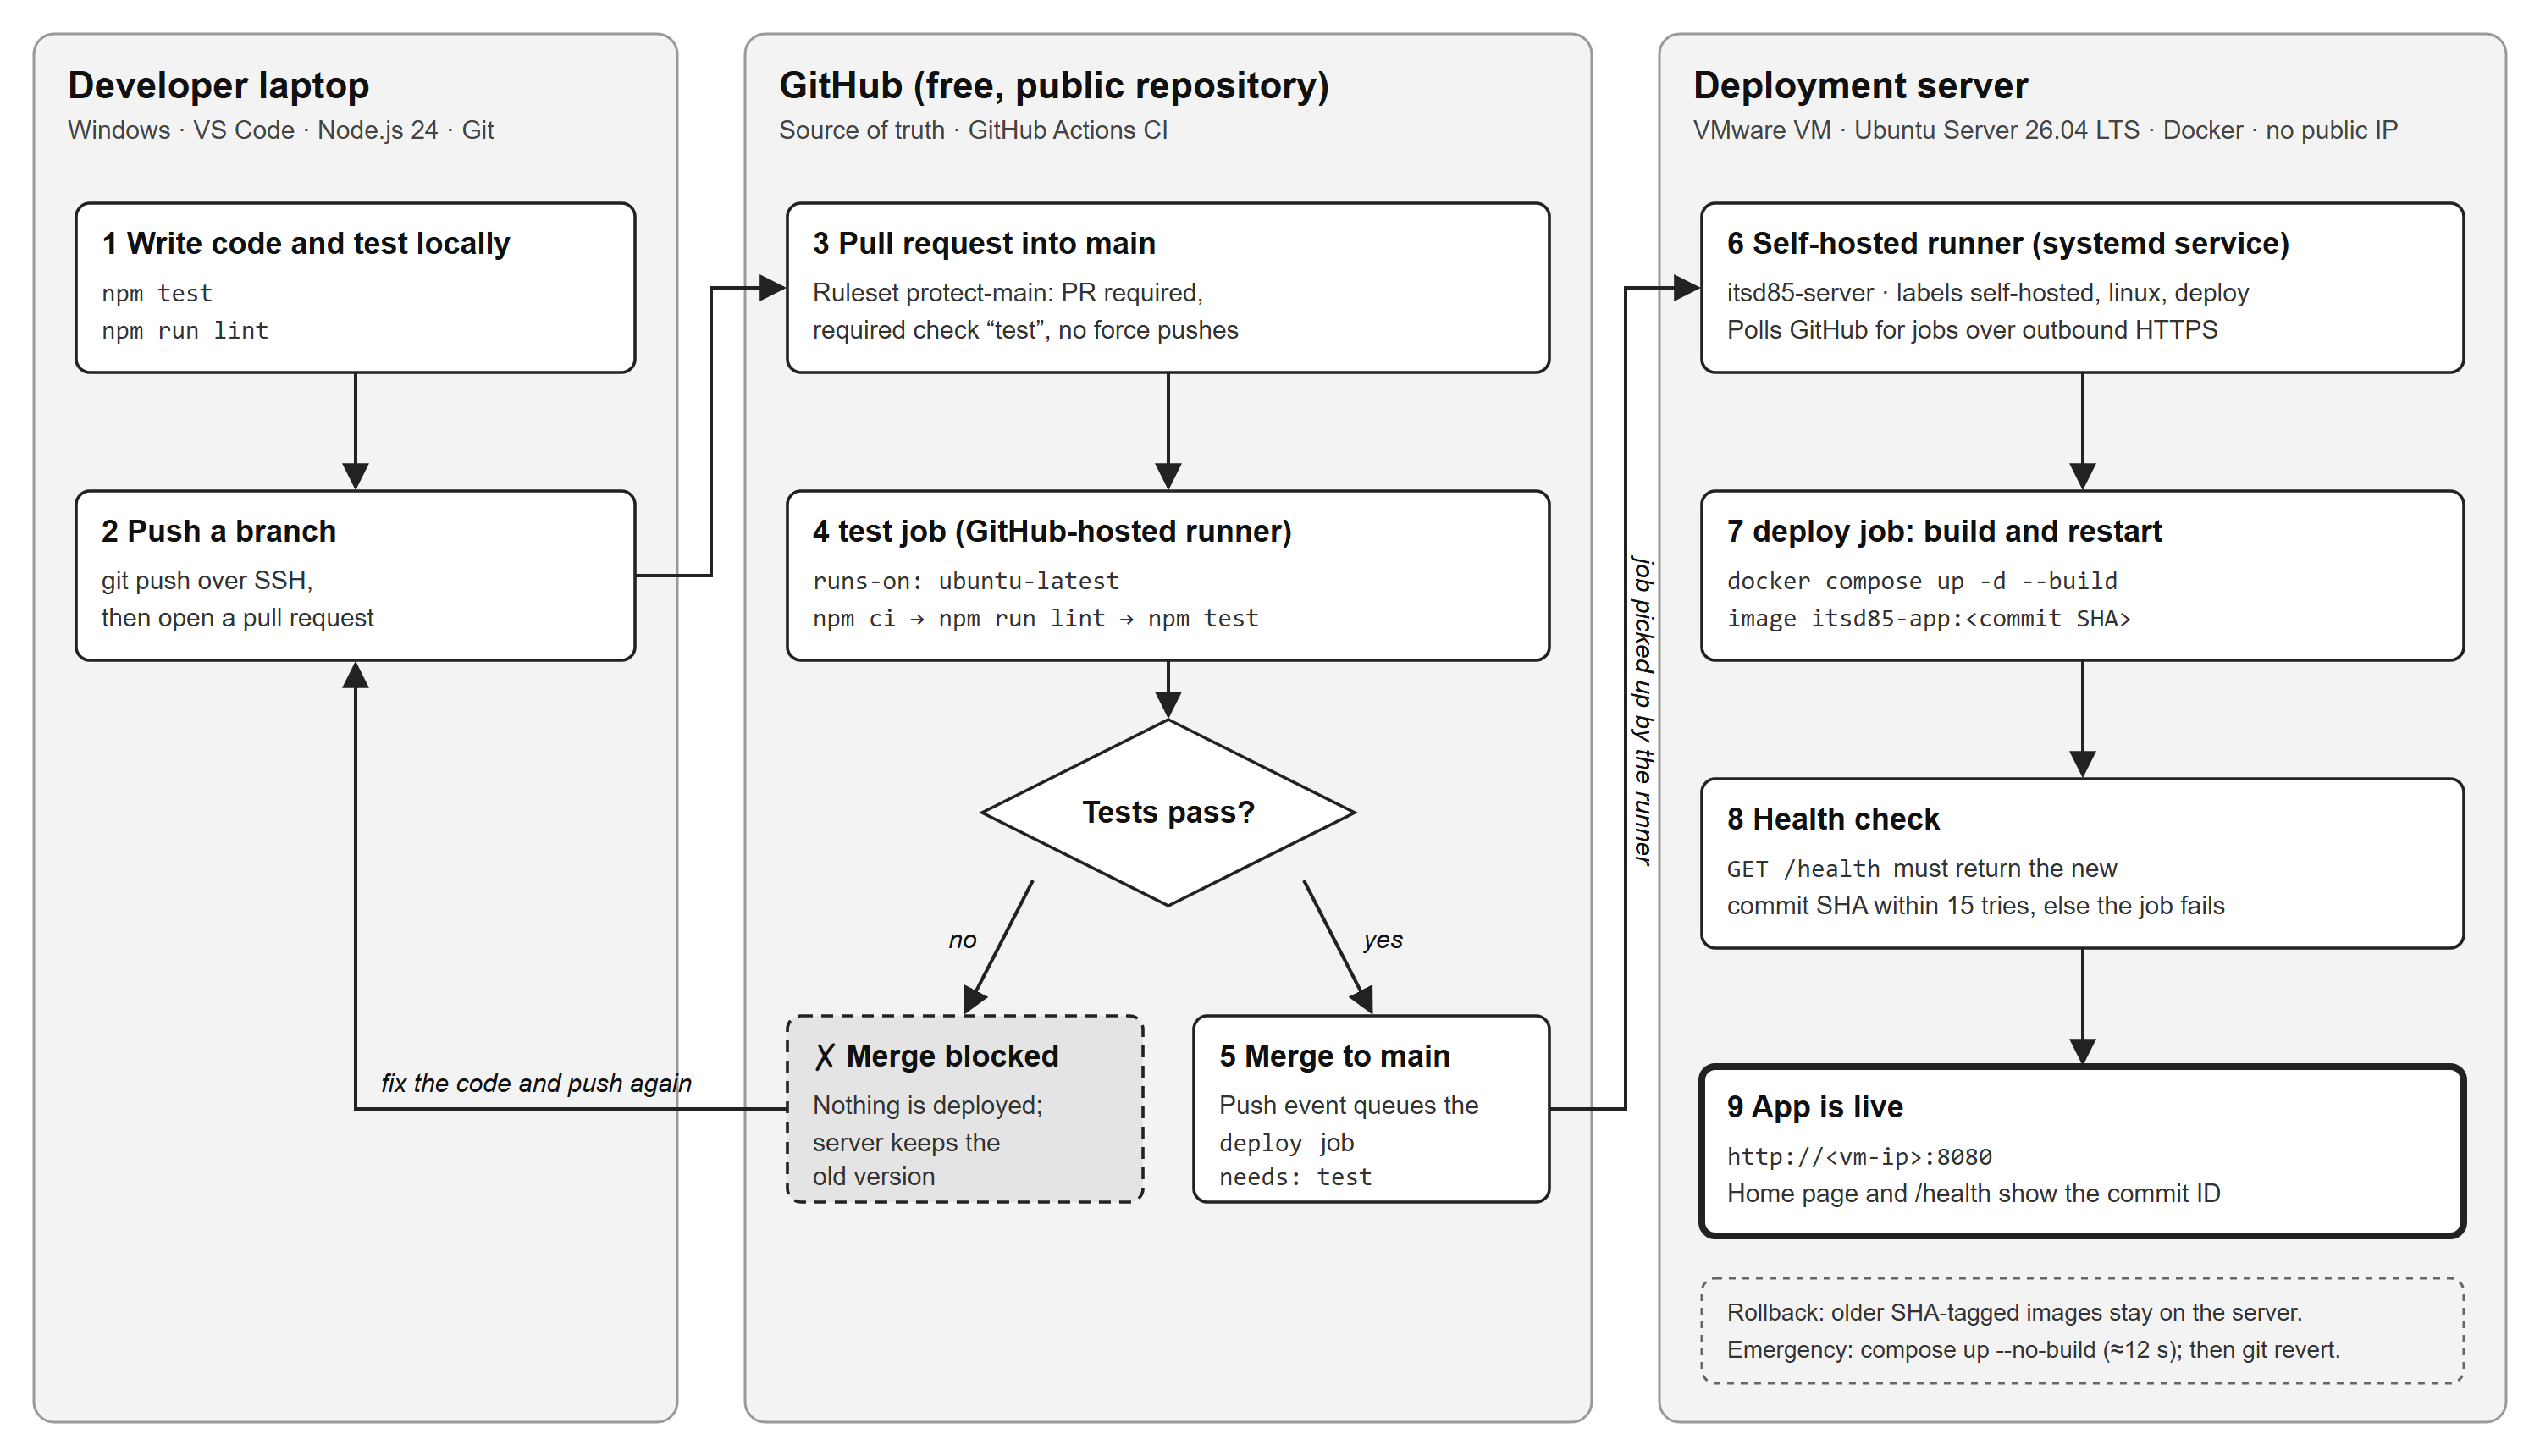
\includegraphics[width=0.92\textwidth]{pipeline.png}
\caption{Pipeline architecture. A change reaches the deployment server only after the test job passes on the protected main branch; the server's runner pulls the deploy job over an outbound connection.}
\label{fig:pipeline}
\end{figure*}

The application is a small Express web API with three routes: a home page, a \texttt{/health} endpoint and an \texttt{/api/add} endpoint. The running version is read from the \texttt{APP\_VERSION} environment variable and shown on the home page and in the \texttt{/health} response, so the deployed commit can be read from any browser. Three automated tests use Node.js's built-in test runner: a unit test of the \texttt{add()} function and two HTTP tests that start the server on a random free port. ESLint checks the code for errors before the tests run.

The laptop is used only to write code, run the tests locally and push branches over SSH. GitHub stores the code and runs the workflow. The main branch is protected by a repository ruleset that requires a pull request and a passing \texttt{test} check before merging, and blocks force pushes.

The deployment server is an Ubuntu Server 26.04 LTS virtual machine in VMware Workstation, using NAT networking with two virtual CPUs and 3.3~GiB of usable memory. It runs Docker Engine with the Compose plugin and the GitHub Actions runner, installed as a systemd service so that it starts when the machine boots. The runner opens an outbound HTTPS connection to GitHub and asks for jobs, so GitHub never needs to connect into the virtual machine. This is why a server behind NAT, with no public IP address, can still receive deployments.

Table~\ref{tab:tools} lists the tools and the paid products they replace. The only tool that is not open source is VMware Workstation, which is free for personal use; the laboratory sheet's VirtualBox works in the same way.

\begin{table}[t]
\caption{Tools Used and the Paid Products They Replace}
\label{tab:tools}
\centering
\footnotesize
\begin{tabular}{@{}L{1.55cm}L{3.15cm}L{2.85cm}@{}}
\toprule
\textbf{Layer} & \textbf{Free tool} & \textbf{Paid alternative}\\
\midrule
Editor & VS Code & JetBrains IDEs\\
Version control & Git, GitHub Free (public repo) & GitHub Team, Bitbucket paid\\
Runtime / tests & Node.js 24, \texttt{node:test} & Paid test services\\
Lint & ESLint & SonarCloud paid tiers\\
CI & GitHub Actions, GitHub-hosted runner & CircleCI, Travis CI paid plans\\
CD agent & GitHub Actions self-hosted runner & Paid cloud deploy services\\
Virtualization & VMware Workstation (free for personal use) & Cloud VPS\\
Server OS & Ubuntu Server 26.04 LTS & Windows Server\\
Containers & Docker Engine, Docker Compose & Docker Desktop business license, Heroku\\
\bottomrule
\end{tabular}
\end{table}

%=====================================================================
\section{Implementation}
The whole pipeline is defined in one workflow file, \texttt{.github/workflows/ci-cd.yml}, with two jobs.

\textbf{Test job.} The \texttt{test} job runs on every push and every pull request to main on a GitHub-hosted \texttt{ubuntu-latest} machine, which is created fresh for each run and deleted afterwards. It checks out the code, installs Node.js~24, installs dependencies with \texttt{npm ci}, runs ESLint and runs the tests. \texttt{npm ci} installs exactly the versions recorded in \texttt{package-lock.json}, so CI tests the same dependency versions the developer used. If any step fails, the job fails.

\textbf{Deploy job and quality gate.} Listing~\ref{lst:deploy} shows the \texttt{deploy} job. The line \texttt{needs: test} is the quality gate: the job starts only if the test job succeeded. The \texttt{if:} condition limits deployment to pushes to main, so pull requests are tested but never deployed. The \texttt{runs-on} labels send the job to the student's own runner, and the \texttt{concurrency} group prevents two deployments from running at the same time.

\begin{lstlisting}[caption={Deploy job of the workflow (health-check loop shortened).},label={lst:deploy},float=t]
deploy:
  needs: test              # quality gate
  if: github.event_name == 'push' && github.ref == 'refs/heads/main'
  runs-on: [self-hosted, linux, deploy]
  concurrency: { group: production, cancel-in-progress: false }
  env:
    APP_VERSION: ${{ github.sha }}   # commit ID = app version
  steps:
    - uses: actions/checkout@v7
    - run: docker compose -p itsd85 up -d --build --remove-orphans
    - name: Health check
      run: |
        for i in $(seq 1 15); do
          curl -fs http://localhost:8080/health | grep -q "$APP_VERSION" && exit 0
          sleep 2
        done
        docker compose -p itsd85 logs --tail 50; exit 1
    - if: always()
      run: docker image prune -f
\end{lstlisting}

\textbf{Versioned images.} The commit ID is passed to Docker Compose as \texttt{APP\_VERSION}. It becomes both a build argument baked into the image and the image tag, \texttt{itsd85-app:<commit ID>}. Each release is therefore an immutable image named after the code it contains. The Dockerfile uses the \texttt{node:24-alpine} base image, installs only production dependencies and runs the application as the unprivileged \texttt{node} user.

\textbf{Health check.} After the container restarts, the job requests \texttt{/health} up to 15 times, two seconds apart, and succeeds only when the response contains the new commit ID. A container that starts and then crashes, or an old container that is still answering, both make the job fail, and the last 50 lines of the container log are printed for diagnosis. A green deploy job therefore means that the new version is confirmed to be live, not only that a command was run.

\textbf{Rollback design.} Because \texttt{docker image prune -f} removes only untagged layers, the images of earlier commits stay on the server. Two rollback methods were implemented. Method~1 reverts the faulty commit with \texttt{git revert}, sends the revert through a pull request, and lets the pipeline deploy it as a new version. Method~2 is an emergency rollback on the server: \texttt{docker compose up -d --no-build} with \texttt{APP\_VERSION} set to an earlier commit ID restarts that commit's image without building anything. Method~2 must be followed by Method~1; otherwise the next deployment brings the faulty code back.

\textbf{Security.} A self-hosted runner executes code from the repository on the student's machine. Because the repository is public, the repository setting that requires approval before workflows from outside contributors' fork pull requests can run was enabled~\cite{ghrunners,ghsecurity}. No server credentials are stored in GitHub, and the runner token used at registration was not committed.

%=====================================================================
\section{Evaluation}
\subsection{Procedure}
Three end-to-end tests from the laboratory activity were carried out on November~23, 2026, after branch protection was enabled. In \textbf{Test A}, a good change (the page title was personalized) was made on a feature branch, opened as a pull request and merged. In \textbf{Test B}, a bug was introduced on purpose by changing \texttt{a + b} to \texttt{a - b} in \texttt{add()}, and a pull request was opened. In \textbf{Test C}, a release that passed the tests but had a visibly wrong page title was merged and deployed, then rolled back first with Method~2 and then with Method~1. All job timings were taken from the GitHub Actions run history. Push-to-live time (lead time) was measured as the duration of the workflow run triggered by the merge, from the push to main until the deploy job's health check passed.

\subsection{Results}
Table~\ref{tab:results} summarizes the three tests. Test~A deployed automatically, and the new title and commit ID appeared on the server 53~s after the merge. In Test~B, the test job failed on \texttt{add() sums two numbers} (expected 5, received $-1$), the ruleset disabled the merge button, and the server continued to serve the Test~A version. In Test~C, the faulty release deployed in 54~s. Method~2 restored the previous commit's image in 12.4~s, measured with \texttt{time} on the server. Method~1 then deployed the revert as a new version 68~s after its merge.

\begin{table}[t]
\caption{End-to-End Test Results}
\label{tab:results}
\centering
\footnotesize
\begin{tabular}{@{}L{1.45cm}L{4.1cm}L{1.6cm}@{}}
\toprule
\textbf{Test} & \textbf{Observed result} & \textbf{Push-to-live}\\
\midrule
A -- good change & test passed (7~s), deploy passed (39~s); new title and commit ID live & 53~s\\
B -- broken change & test failed ($-1 \neq 5$); merge blocked; server unchanged & n/a\\
C -- Method 1 & revert merged; old content live under a new commit ID & 68~s\\
C -- Method 2 & previous commit's image restarted, no rebuild & 12.4~s\\
\bottomrule
\end{tabular}
\end{table}

Fig.~\ref{fig:times} breaks down all six deployments, which include the first deployment, Tests~A and C, and two documentation changes. The mean push-to-live time was 56.5~s (median 54~s, range 52--68~s, $n = 6$). The deploy job was the largest part and was very stable, with a mean of 39.7~s (range 39--42~s). The test job took a mean of 9.7~s (range 7--18~s), and the self-hosted runner picked up the deploy job 4--5~s after the test job finished. The slowest run, at 68~s, was caused mainly by an 18~s test job on the GitHub-hosted runner. On the six pull-request runs, the test job took a mean of 8.8~s to report a result.

\begin{figure}[t]
\centering
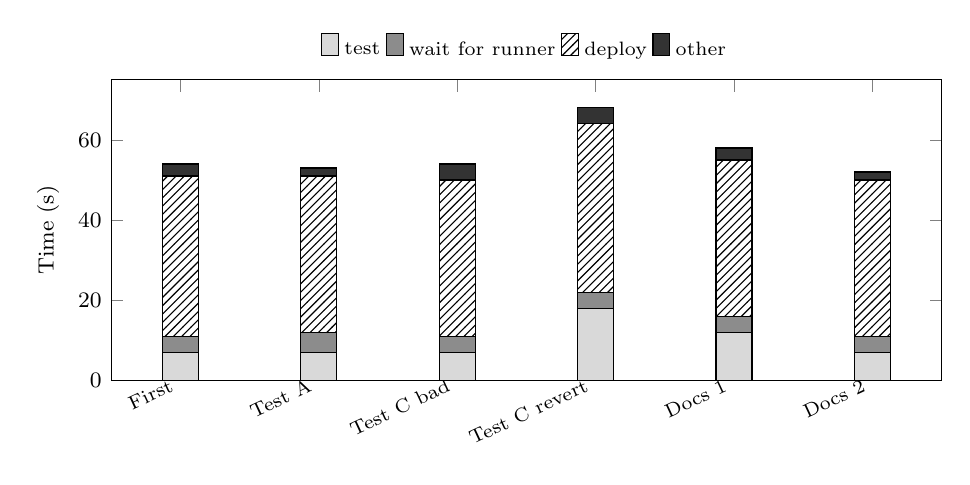
\begin{tikzpicture}
\begin{axis}[
  ybar stacked, bar width=13pt, width=\columnwidth, height=5.4cm,
  ymin=0, ymax=75, ylabel={Time (s)}, ylabel style={font=\footnotesize},
  symbolic x coords={D1,D2,D3,D4,D5,D6},
  xtick=data, xticklabels={{First},{Test A},{Test C bad},{Test C revert},{Docs 1},{Docs 2}},
  x tick label style={font=\scriptsize, rotate=25, anchor=east},
  y tick label style={font=\footnotesize},
  legend style={font=\scriptsize, at={(0.5,1.03)}, anchor=south, legend columns=4, draw=none},
  nodes near coords style={font=\scriptsize},
]
\addplot[fill=black!15, draw=black] coordinates {(D1,7) (D2,7) (D3,7) (D4,18) (D5,12) (D6,7)};
\addplot[fill=black!45, draw=black] coordinates {(D1,4) (D2,5) (D3,4) (D4,4) (D5,4) (D6,4)};
\addplot[fill=white, draw=black, postaction={pattern=north east lines}] coordinates {(D1,40) (D2,39) (D3,39) (D4,42) (D5,39) (D6,39)};
\addplot[fill=black!80, draw=black] coordinates {(D1,3) (D2,2) (D3,4) (D4,4) (D5,3) (D6,2)};
\legend{test, wait for runner, deploy, other}
\end{axis}
\end{tikzpicture}
\caption{Push-to-live time of each deployment, split into the test job, the wait for the self-hosted runner, the deploy job and other workflow overhead. Totals: 54, 53, 54, 68, 58 and 52~s.}
\label{fig:times}
\end{figure}

Across all 14 workflow runs, the one change with a failing test was the only change blocked, and it never reached the server. The faulty release in Test~C passed all tests and was deployed, so the change failure rate over the six deployments was 1 in 6. That failure was deliberate, but it shows a real limit of the gate.

%=====================================================================
\section{Discussion}
The pipeline did what it was designed to do. Every merge to main was live and verified about one minute later without the developer touching the server, and the commit ID on the page made it possible to confirm which code was running at any moment. The quality gate worked at the point where it matters most: a failing test made the merge button unusable, so the broken change could not reach main or the server.

Test~C exposed the main limitation: the gate is only as good as the tests. A release with a wrong title passed three tests that never checked the title. In this situation the commit-tagged images were the most useful design choice, because they turned recovery into restarting a container (12.4~s) instead of rebuilding the application. The revert through the pipeline took longer (68~s after merge, plus the time to open and review the pull request), but it was the only fix that also corrected main.

Other limitations follow from the setup. The virtual machine must be running for deployments to happen; while it is off, deploy jobs wait in the queue. There is a single server and no staging environment, so a release is tested on production directly. A self-hosted runner on a public repository is a security risk, because pull-request code could run on the student's machine. Here this was reduced by requiring approval for outside contributors and by never deploying pull requests. Finally, the server's logical volume used only 11.2~GB of the 25~GB virtual disk, and each deployment keeps an image of about 255~MB, so old images must be removed periodically.

The evaluation also has threats to validity. The sample was small (six deployments, one application and one server) and all measurements were taken on one day on one laptop, so the times may differ on other hardware or networks. The first build on the server also downloaded the base image, while later builds reused cached layers. The application is very small, so build and test times for real projects will be longer, although the overhead added by the pipeline itself, about 4--5~s to pick up a job, should not grow.

%=====================================================================
\section{Conclusion and Future Work}
\textbf{RQ1:} Yes. A toolchain of free tools (Git, GitHub Actions, a self-hosted runner, Docker and an Ubuntu virtual machine) automatically tested and deployed every change from a student laptop to a server that has no public IP address.

\textbf{RQ2:} The mean lead time from merge to a verified live release was 56.5~s over six deployments (range 52--68~s). Time to restore was 12.4~s with the emergency image rollback and 68~s after merging a revert through the pipeline.

\textbf{RQ3:} The required test check blocked the only change with a failing test, so no failing change reached the server. A release whose defect was not covered by any test was deployed, showing that the gate depends on test coverage.

Future work includes a staging environment deployed from a \texttt{develop} branch before production, a test-coverage threshold in CI, building the image once in CI and publishing it to the GitHub Container Registry instead of building on the server, deployment notifications to a class chat channel, and a fully self-hosted version using Forgejo or Gitea with their Actions-compatible runners.

%=====================================================================
\section*{Acknowledgment}
The author thanks the ITSD~85 instructor for the laboratory design. Claude (Anthropic), an AI assistant, was used to help write the sample application, workflow and documentation, to collect run timings from the GitHub API, and to suggest wording for this paper; all measurements come from the author's own pipeline runs, and the author reviewed and is responsible for the content.

\begin{thebibliography}{00}
\bibitem{humble2010} J. Humble and D. Farley, \textit{Continuous Delivery: Reliable Software Releases through Build, Test, and Deployment Automation}. Boston, MA, USA: Addison-Wesley, 2010.
\bibitem{fowler2006} M. Fowler, ``Continuous integration,'' martinfowler.com, May 2006. [Online]. Available: \url{https://martinfowler.com/articles/continuousIntegration.html}
\bibitem{chen2015} L. Chen, ``Continuous delivery: Huge benefits, but challenges too,'' \textit{IEEE Softw.}, vol. 32, no. 2, pp. 50--54, 2015.
\bibitem{shahin2017} M. Shahin, M. Ali Babar, and L. Zhu, ``Continuous integration, delivery and deployment: A systematic review on approaches, tools, challenges and practices,'' \textit{IEEE Access}, vol. 5, pp. 3909--3943, 2017.
\bibitem{hilton2016} M. Hilton, T. Tunnell, K. Huang, D. Marinov, and D. Dig, ``Usage, costs, and benefits of continuous integration in open-source projects,'' in \textit{Proc. 31st IEEE/ACM Int. Conf. Automated Softw. Eng. (ASE)}, 2016, pp. 426--437.
\bibitem{zampetti2021} F. Zampetti, S. Geremia, G. Bavota, and M. Di Penta, ``CI/CD pipelines evolution and restructuring: A qualitative and quantitative study,'' in \textit{Proc. IEEE Int. Conf. Softw. Maintenance Evol. (ICSME)}, 2021, pp. 471--482. % VERIFY pages
\bibitem{kinsman2021} T. Kinsman, M. Wessel, M. A. Gerosa, and C. Treude, ``How do software developers use GitHub Actions to automate their workflows?'' in \textit{Proc. IEEE/ACM 18th Int. Conf. Mining Softw. Repositories (MSR)}, 2021, pp. 420--431.
\bibitem{decan2022} A. Decan, T. Mens, P. R. Mazrae, and M. Golzadeh, ``On the use of GitHub Actions in software development repositories,'' in \textit{Proc. IEEE Int. Conf. Softw. Maintenance Evol. (ICSME)}, 2022, pp. 235--245. % VERIFY pages
\bibitem{wessel2023} M. Wessel, J. Vargovich, M. A. Gerosa, and C. Treude, ``GitHub Actions: The impact on the pull request process,'' \textit{Empirical Softw. Eng.}, vol. 28, no. 6, Art. no. 131, 2023. % VERIFY volume, issue and article number
\bibitem{forsgren2018} N. Forsgren, J. Humble, and G. Kim, \textit{Accelerate: The Science of Lean Software and DevOps}. Portland, OR, USA: IT Revolution, 2018.
\bibitem{dora2024} DORA, Google Cloud, ``Accelerate State of DevOps Report 2024,'' 2024. [Online]. Available: \url{https://dora.dev/research/2024/dora-report/}
\bibitem{merkel2014} D. Merkel, ``Docker: Lightweight Linux containers for consistent development and deployment,'' \textit{Linux J.}, vol. 2014, no. 239, Art. no. 2, 2014.
\bibitem{christensen2016} H. B. Christensen, ``Teaching DevOps and cloud computing using a cognitive apprenticeship and story-telling approach,'' in \textit{Proc. ACM Conf. Innovation Technol. Comput. Sci. Educ. (ITiCSE)}, 2016, pp. 174--179.
\bibitem{fernandes2022} M. Fernandes, S. Ferino, A. Fonseca, L. Fonseca, U. Kulesza, and E. Aranha, ``DevOps education: An interview study of challenges and recommendations,'' in \textit{Proc. IEEE/ACM 44th Int. Conf. Softw. Eng.: Softw. Eng. Educ. Training (ICSE-SEET)}, 2022, pp. 90--101.
\bibitem{ghrunners} GitHub, ``About self-hosted runners,'' \textit{GitHub Docs}. [Online]. Available: \url{https://docs.github.com/en/actions/hosting-your-own-runners/managing-self-hosted-runners/about-self-hosted-runners} (accessed Nov. 23, 2026).
\bibitem{ghsecurity} GitHub, ``Security hardening for GitHub Actions,'' \textit{GitHub Docs}. [Online]. Available: \url{https://docs.github.com/en/actions/security-for-github-actions/security-guides/security-hardening-for-github-actions} (accessed Nov. 23, 2026).
\end{thebibliography}

%=====================================================================
\clearpage
\onecolumn
\appendices
\section{Repository and Release}
\begin{itemize}
\item Repository: \url{https://github.com/Ennius5/itsd85-lab6-bsit4c-Campomanes}
\item Release: \url{https://github.com/Ennius5/itsd85-lab6-bsit4c-Campomanes/releases/tag/v1.0}
\item Workflow runs: \url{https://github.com/Ennius5/itsd85-lab6-bsit4c-Campomanes/actions}
\end{itemize}

\section{Results Table (Laboratory Part 7.5)}
\begin{center}
\small
\begin{tabular}{@{}L{2.6cm}L{4.4cm}L{4.6cm}L{1.6cm}L{3.2cm}@{}}
\toprule
\textbf{Test} & \textbf{Expected result} & \textbf{Actual result} & \textbf{Push-to-live} & \textbf{Screenshots}\\
\midrule
A -- good change & test passes, deploy passes, new name and commit ID live & test 7~s, deploy 39~s; title and commit \texttt{bc6c3ed} live & 0:53 & Figs.~\ref{fig:t7a1}--\ref{fig:t7a2}\\
B -- broken change & test fails, merge blocked, server unchanged & test failed ($-1 \neq 5$); merge blocked; server stayed on \texttt{bc6c3ed} & n/a & Figs.~\ref{fig:t7b1}--\ref{fig:t7b3}\\
C -- rollback (Method 1) & old content and a new commit ID live & revert merged; old title live as \texttt{ff4da10} & 1:08 & Figs.~\ref{fig:t7c1}, \ref{fig:t7c3}, \ref{fig:t7c4}\\
C -- rollback (Method 2) & previous commit ID live within seconds & \texttt{bc6c3ed} live again without a rebuild & 0:12.4 & Fig.~\ref{fig:t7c2}\\
\bottomrule
\end{tabular}
\end{center}

\section{Answers to the Guide Questions}
\textbf{1. CI, continuous delivery and continuous deployment.} Continuous integration means every change is merged into a shared main line often and is built and tested automatically each time. Continuous delivery adds an automated release process, so every change that passes is ready to release, but a person still decides when to release it. Continuous deployment goes one step further and releases every passing change automatically. This lab built continuous deployment: every merge to main that passed the tests went live with no manual step.

\textbf{2. Why does deploy use \texttt{needs: test}?} It makes the deploy job wait for the test job and run only if it succeeded, so it is the quality gate. Without it, both jobs would start at the same time, and a change with failing tests could be deployed before (or regardless of) the test result.

\textbf{3. How could GitHub deploy to a server with no public IP?} GitHub never connected to the server. The self-hosted runner on the server made an outbound HTTPS connection to GitHub and asked for jobs. When a deploy job was queued, the runner picked it up through that connection and ran it locally. Outbound connections work through NAT, so no public IP or port forwarding was needed.

\textbf{4. Why \texttt{npm ci} instead of \texttt{npm install}?} \texttt{npm ci} installs exactly the versions in \texttt{package-lock.json}, starts from a clean \texttt{node\_modules}, and fails if the lock file and \texttt{package.json} do not match. CI therefore tests the same dependency versions the developer used, and builds are repeatable. \texttt{npm install} may resolve newer versions and update the lock file.

\textbf{5. Why use the commit ID as the version?} (a) Traceability: the page and \texttt{/health} show exactly which commit is running, so it can be compared with GitHub, and the health check can prove that the new version is live. (b) Rollback: each image is tagged with its commit ID, so the image of any earlier commit can be restarted directly. It also needs no manual version numbering.

\textbf{6. Rollback Method 1 vs. Method 2.} Method 1 (revert and redeploy through the pipeline) is the normal choice. It fixes main, is tested, and is recorded in Git history, but it took about a minute plus the time to open and merge a pull request. Method 2 (restart the previous image on the server) took 12.4~s and needs no build, so it is for emergencies when users are affected right now. It does not change main, so it must always be followed by Method 1.

\textbf{7. Security risks of a self-hosted runner on a public repository.} Anyone can open a pull request, and a workflow from that pull request could run arbitrary code on the runner, which is the student's own machine with Docker access. To reduce this, approval was required for all outside contributors before fork pull-request workflows can run, the deploy job runs only on pushes to main (never on pull requests), main is protected so changes need a passing pull request, and no secrets or server credentials are stored in GitHub.

\textbf{8. A paid product and its free replacement.} Heroku, a paid platform-as-a-service, builds and hosts an application on each push. In this lab, the GitHub Actions self-hosted runner together with Docker Engine and Docker Compose on a local Ubuntu virtual machine did the same job for free: they built the application into a container and ran it on every push to main.

\section{Screenshots}
\begin{figure}[H]\centering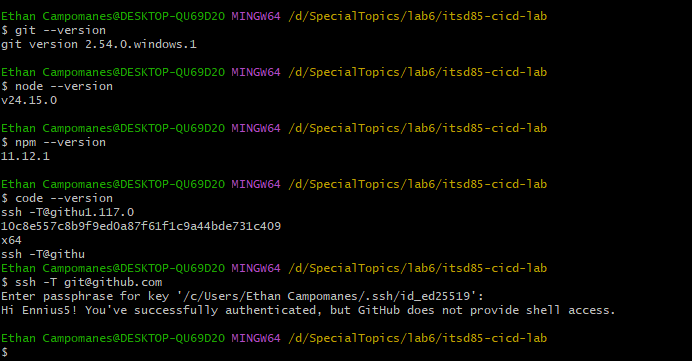
\includegraphics[width=0.75\textwidth]{cp1-versions.png}\caption{Checkpoint 1: Git, Node.js, npm and editor versions, and SSH authentication to GitHub.}\end{figure}
\begin{figure}[H]\centering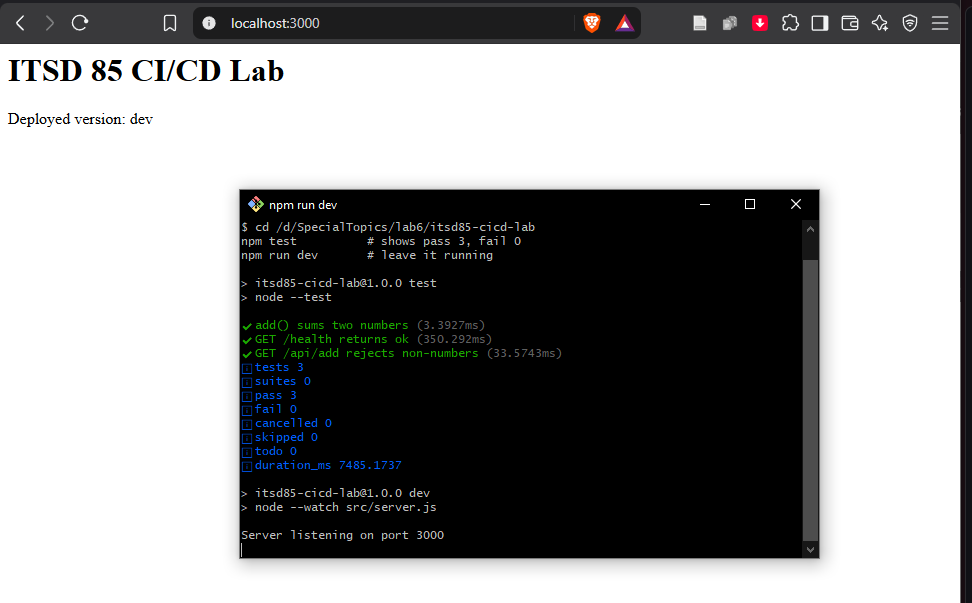
\includegraphics[width=0.75\textwidth]{cp2-tests-and-dev-server.png}\caption{Checkpoint 2: three passing tests and the application running locally (version \texttt{dev}).}\end{figure}
\begin{figure}[H]\centering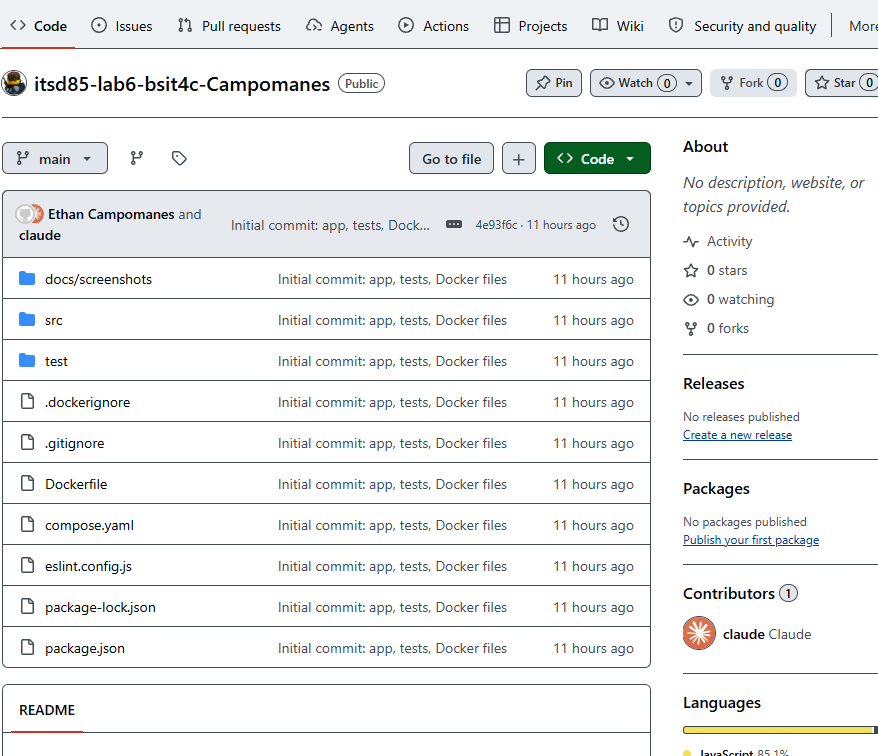
\includegraphics[width=0.7\textwidth]{cp3-repo-files.png}\caption{Checkpoint 3: repository file list on GitHub (no \texttt{node\_modules}).}\end{figure}
\begin{figure}[H]\centering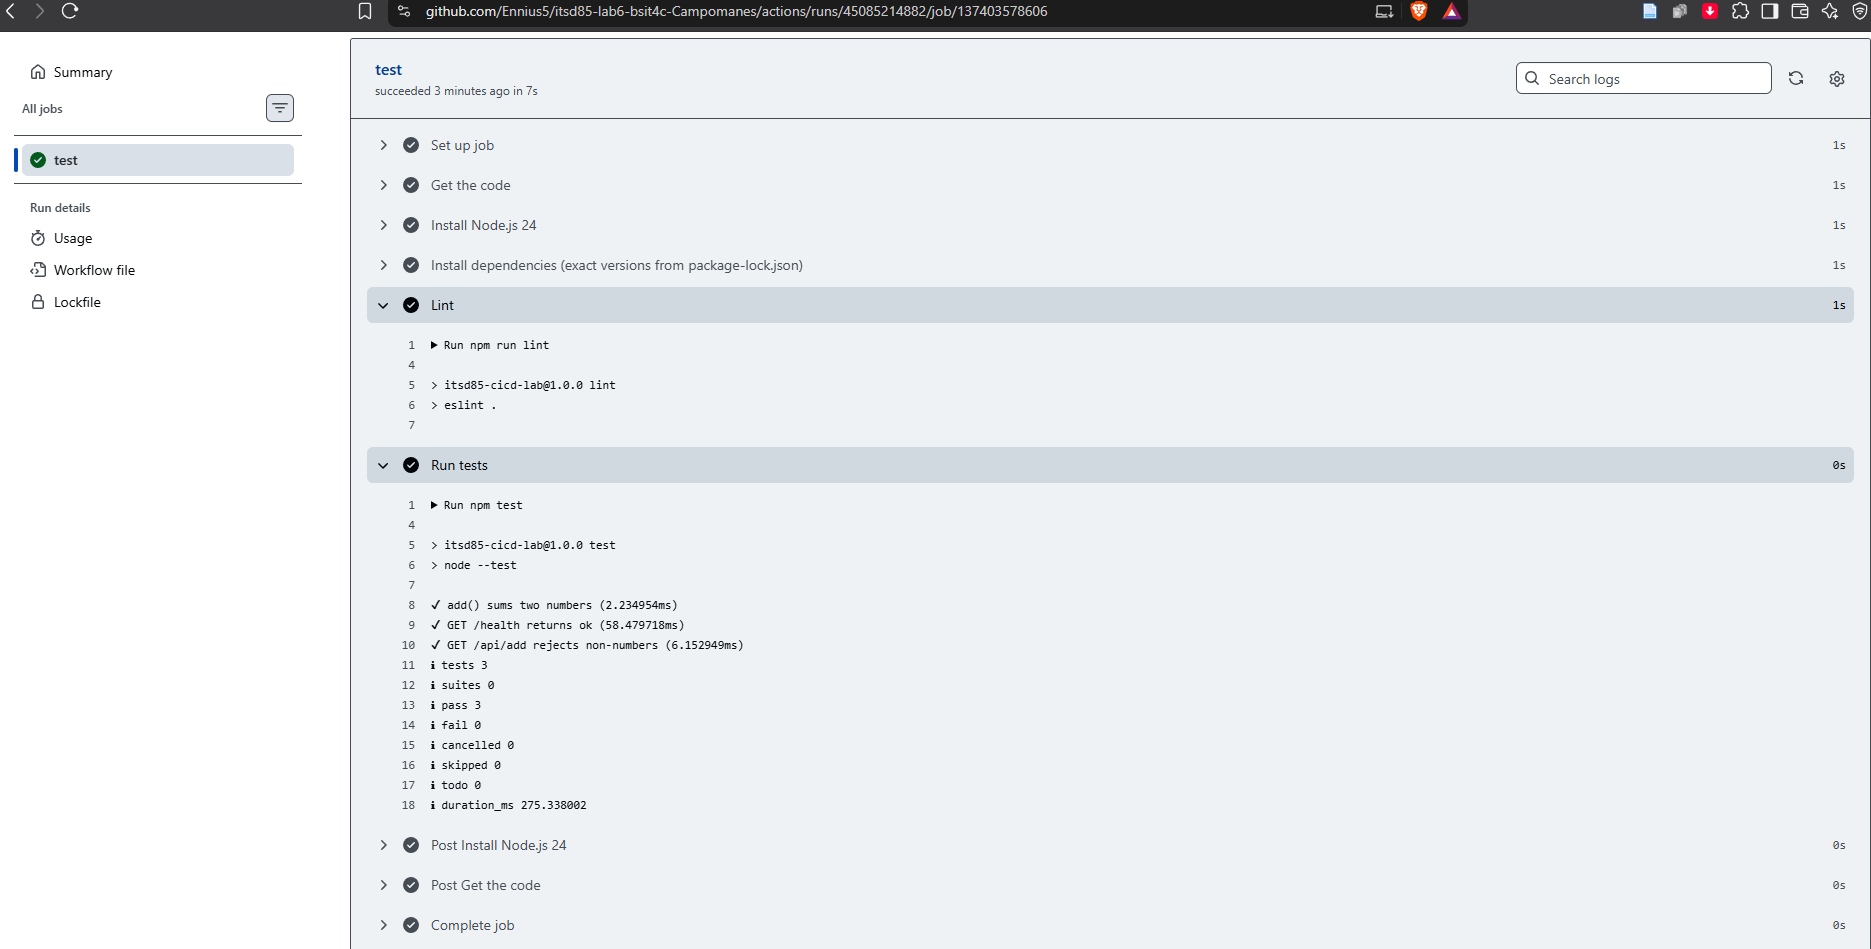
\includegraphics[width=0.95\textwidth]{cp4-ci-green.png}\caption{Checkpoint 4: green test job with the lint and test output.}\end{figure}
\begin{figure}[H]\centering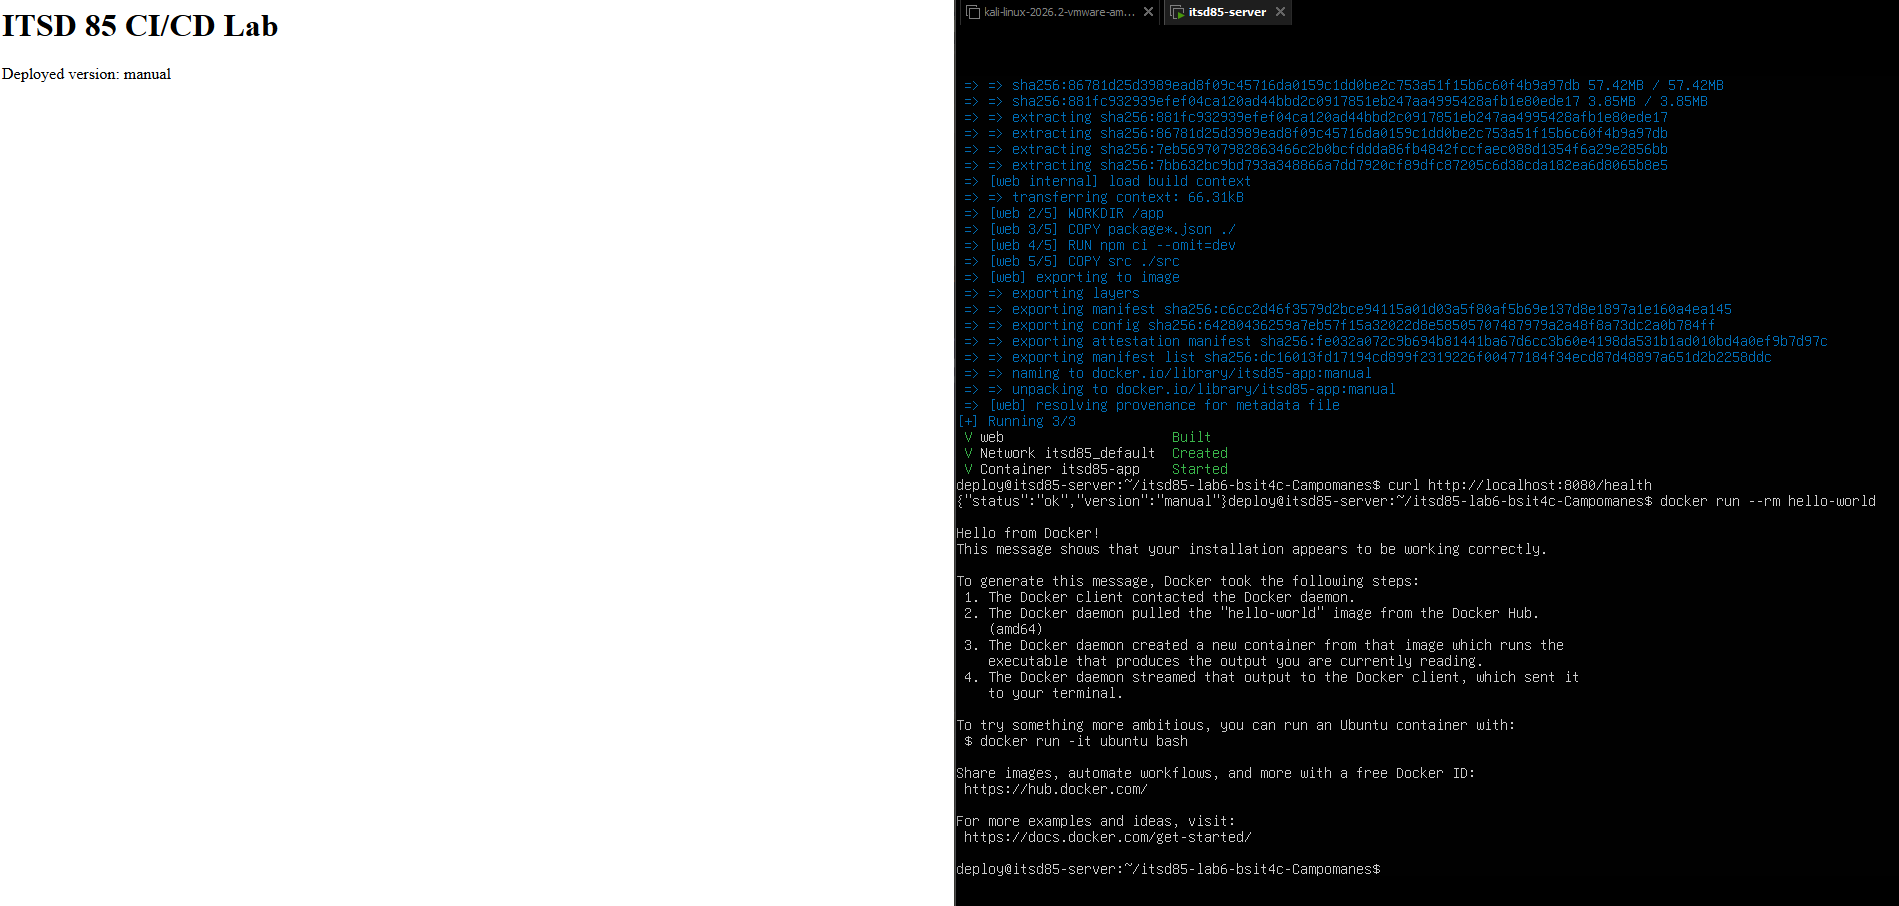
\includegraphics[width=0.95\textwidth]{cp5-hello-world.png}\caption{Checkpoint 5: Docker on the server and the manual deployment (version \texttt{manual}).}\end{figure}
\begin{figure}[H]\centering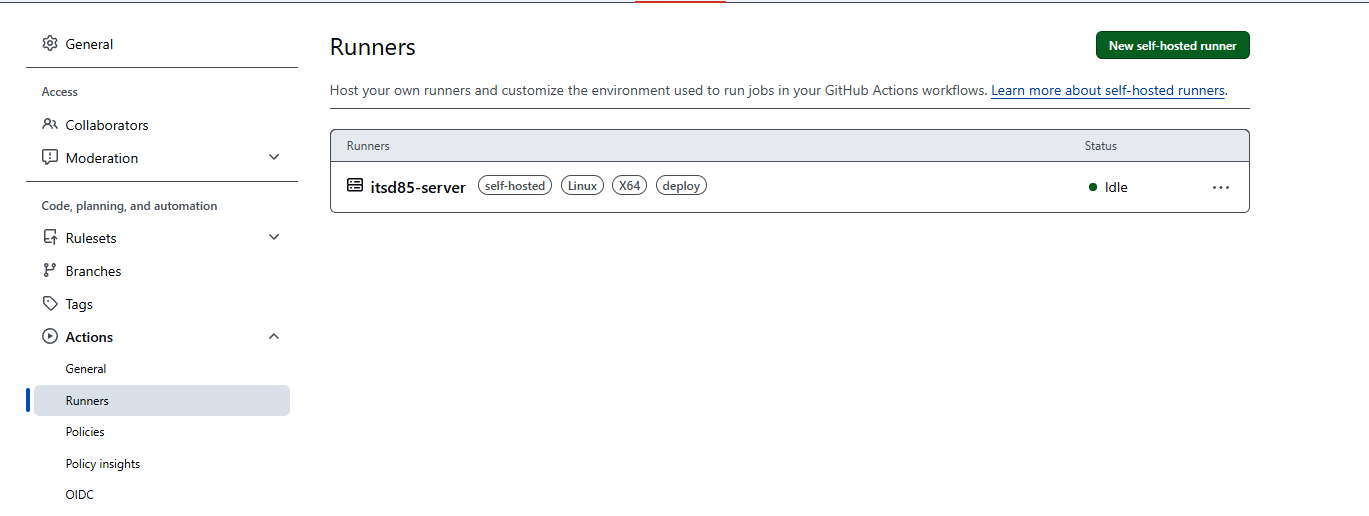
\includegraphics[width=0.9\textwidth]{cp6a-runner-idle.png}\caption{Checkpoint 6a: self-hosted runner \texttt{itsd85-server} idle with the \texttt{deploy} label.}\end{figure}
\begin{figure}[H]\centering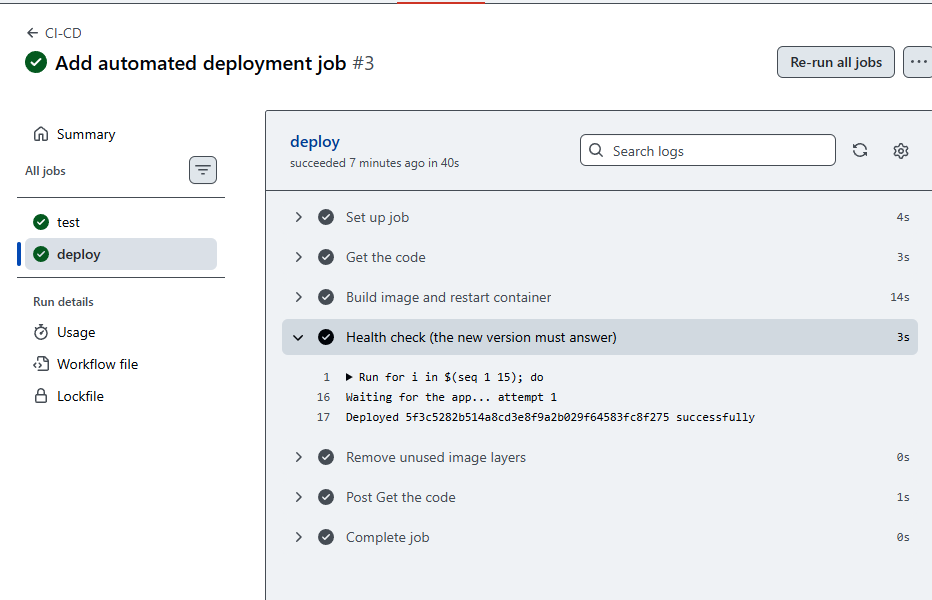
\includegraphics[width=0.95\textwidth]{cp6b-deploy-green.png}\caption{Checkpoint 6b: green test and deploy run.}\end{figure}
\begin{figure}[H]\centering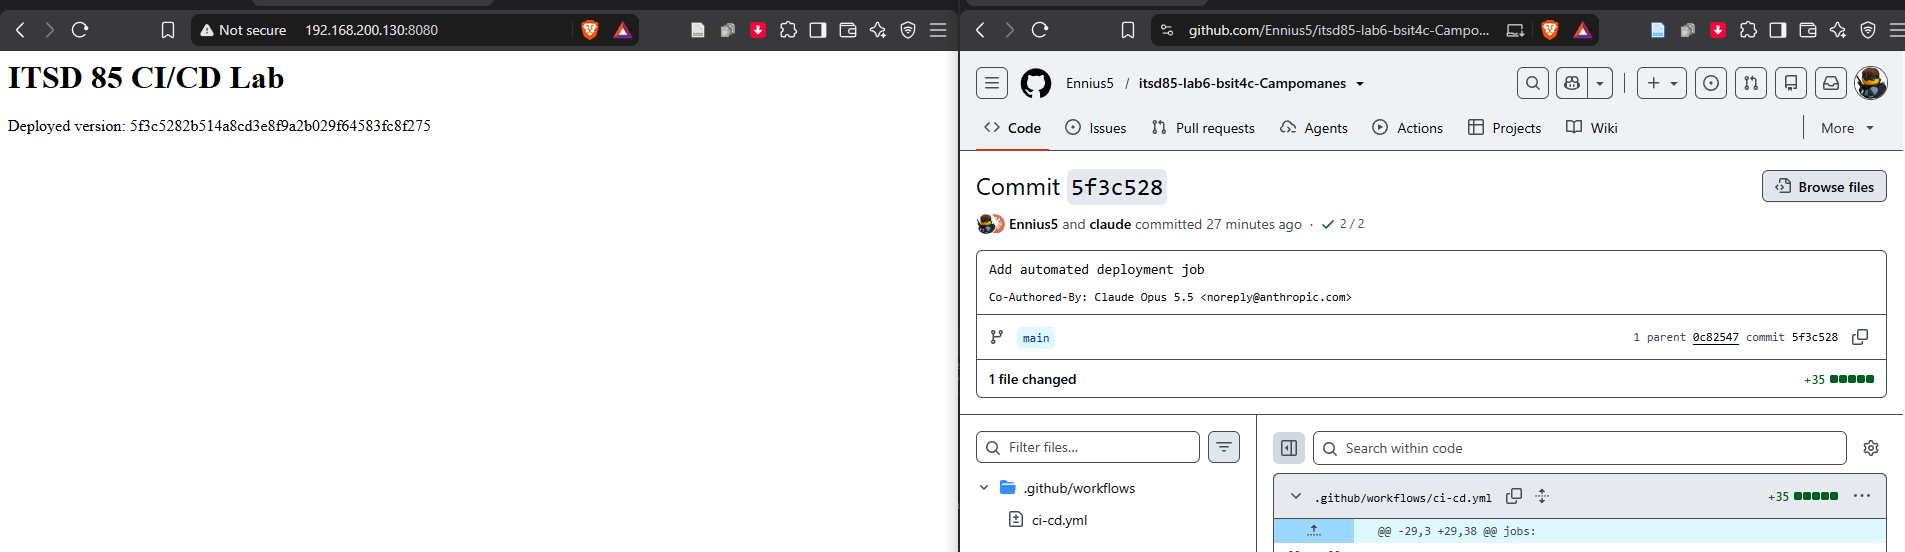
\includegraphics[width=0.95\textwidth]{cp6c-commit-live.png}\caption{Checkpoint 6c: the live commit ID matches the commit on GitHub.}\end{figure}
\begin{figure}[H]\centering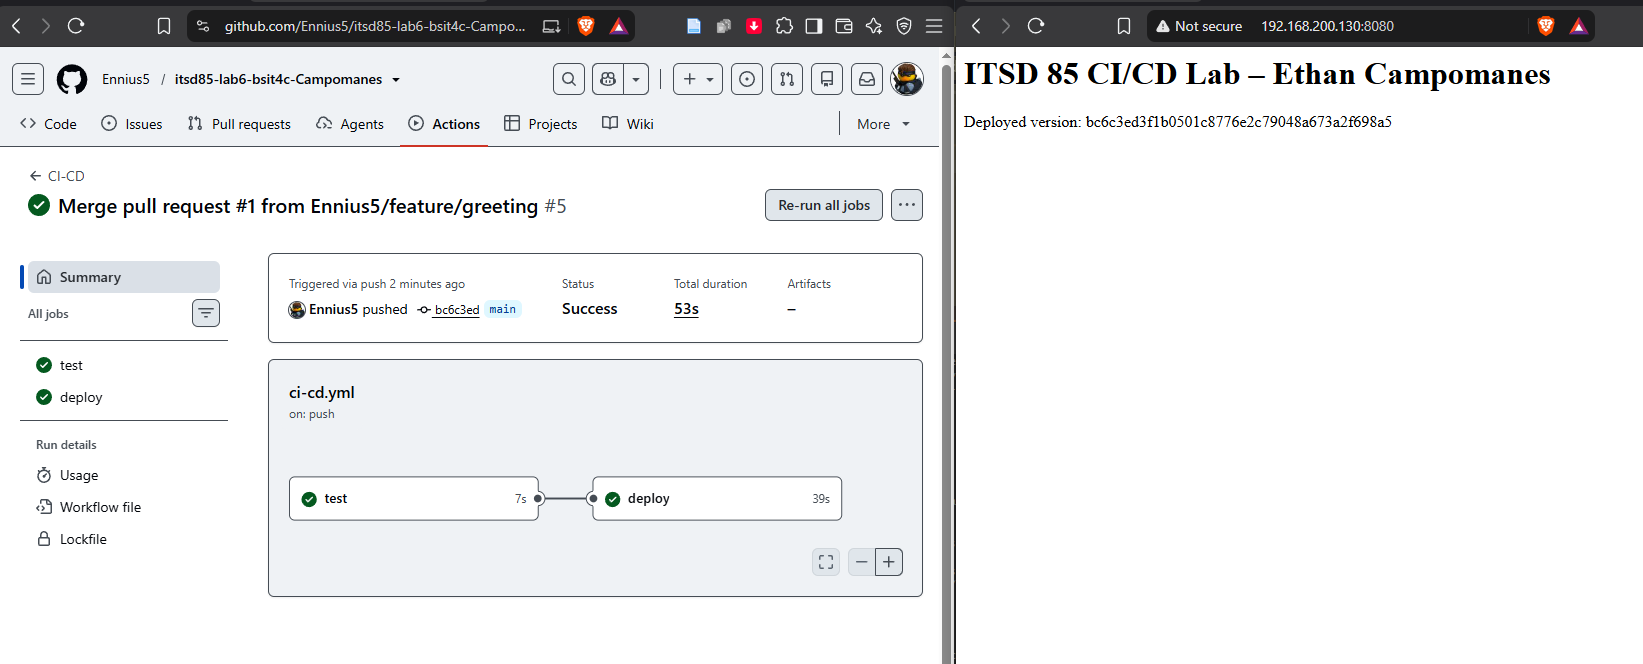
\includegraphics[width=0.8\textwidth]{t7a-pr-green.png}\caption{Test A: pull request with a passing test check.}\label{fig:t7a1}\end{figure}
\begin{figure}[H]\centering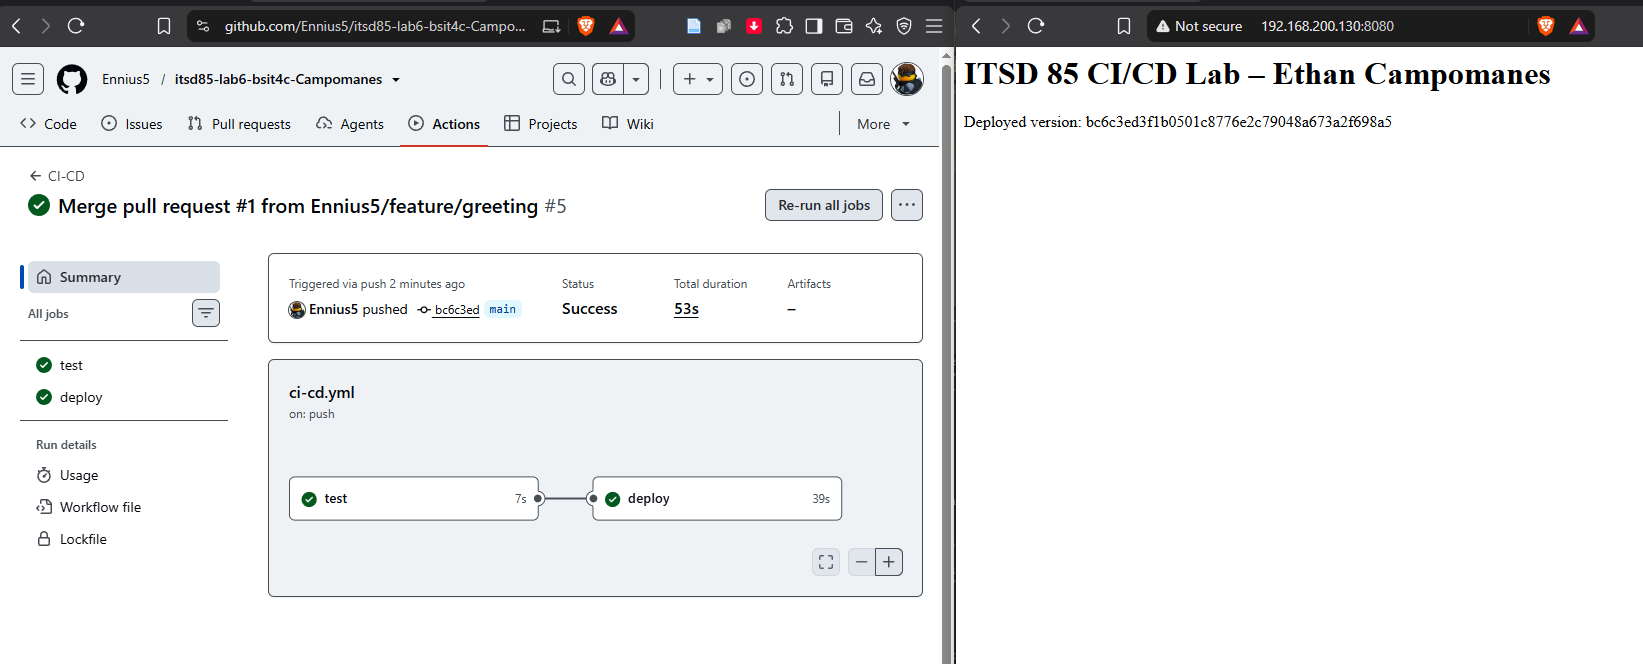
\includegraphics[width=0.95\textwidth]{t7a-live.png}\caption{Test A: test and deploy passed; the new title and commit ID are live.}\label{fig:t7a2}\end{figure}
\begin{figure}[H]\centering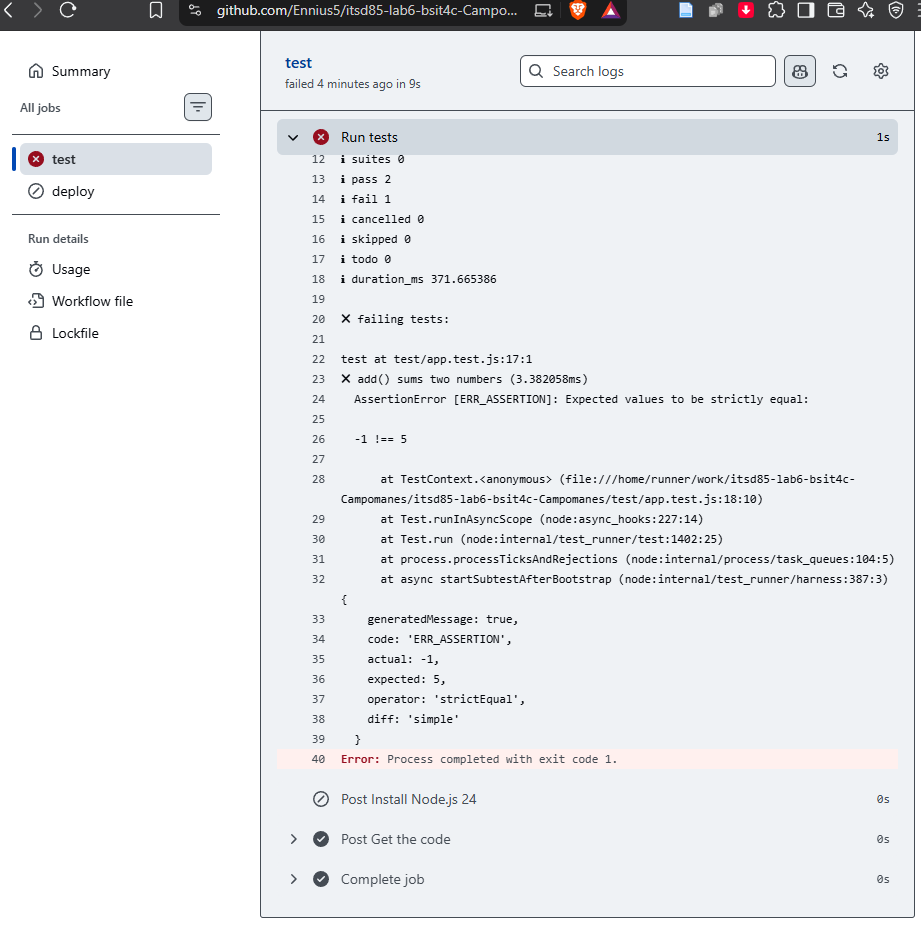
\includegraphics[width=0.8\textwidth]{t7b-test-failed.png}\caption{Test B: \texttt{add() sums two numbers} fails ($-1 \neq 5$).}\label{fig:t7b1}\end{figure}
\begin{figure}[H]\centering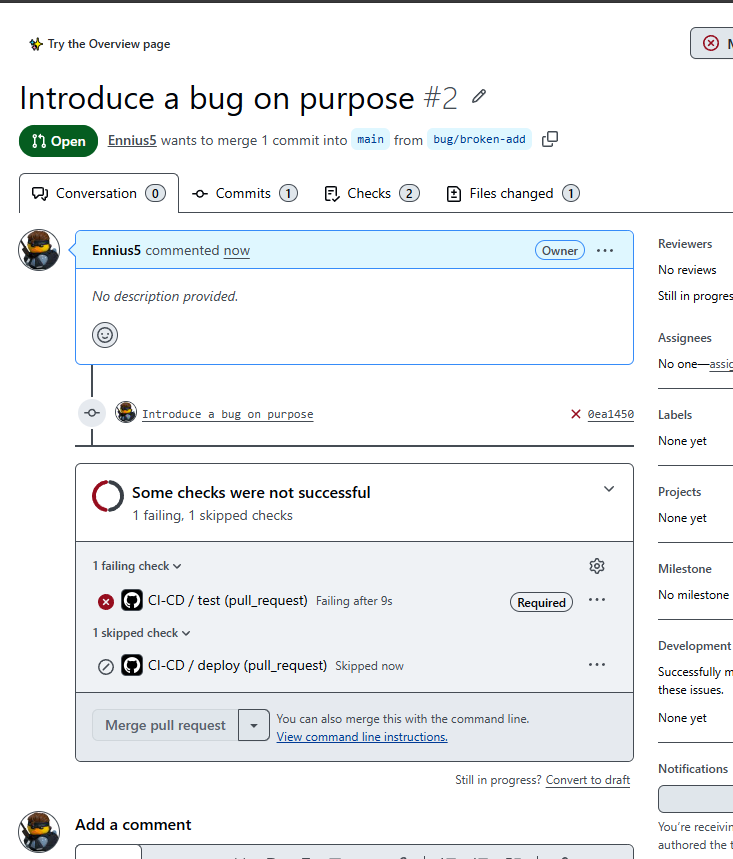
\includegraphics[width=0.6\textwidth]{t7b-merge-blocked.png}\caption{Test B: the required test check failed and the merge is blocked.}\label{fig:t7b2}\end{figure}
\begin{figure}[H]\centering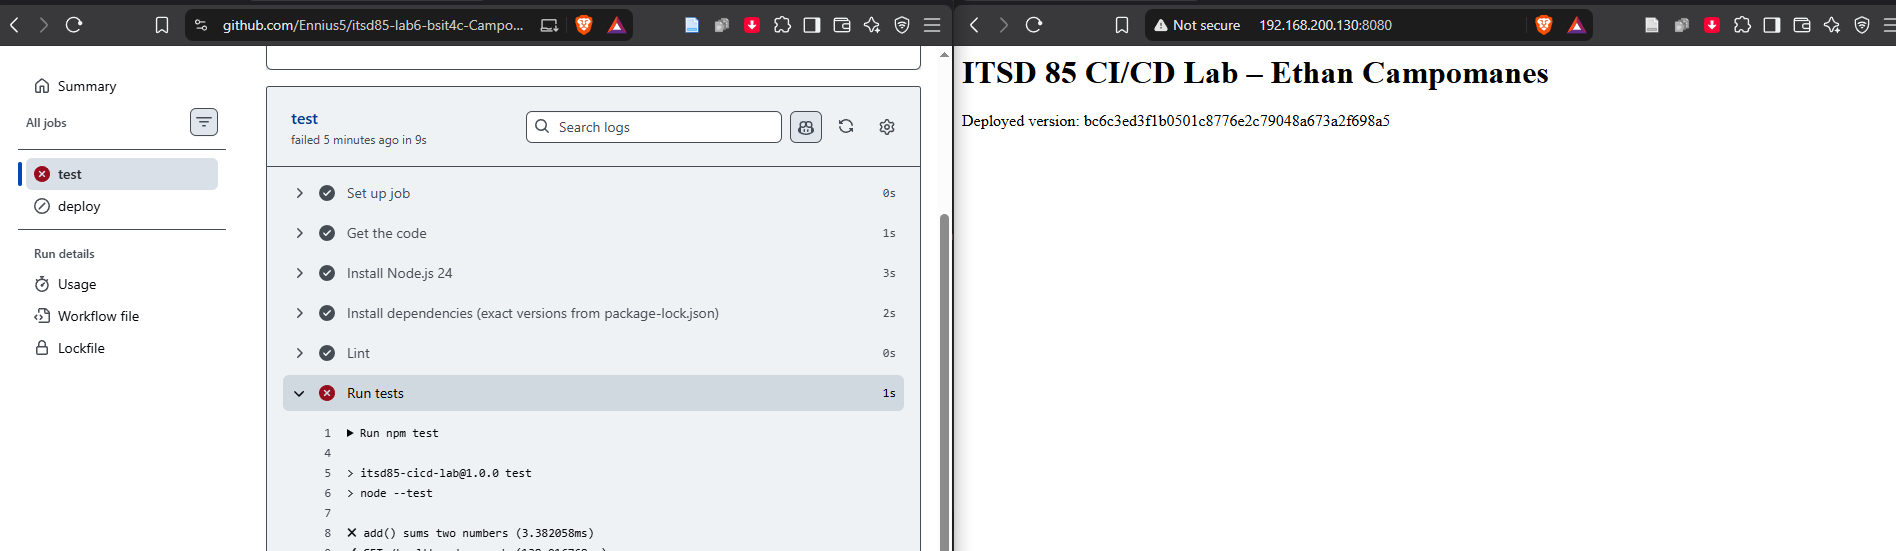
\includegraphics[width=0.95\textwidth]{t7b-server-unchanged.png}\caption{Test B: the server still runs the Test A commit.}\label{fig:t7b3}\end{figure}
\begin{figure}[H]\centering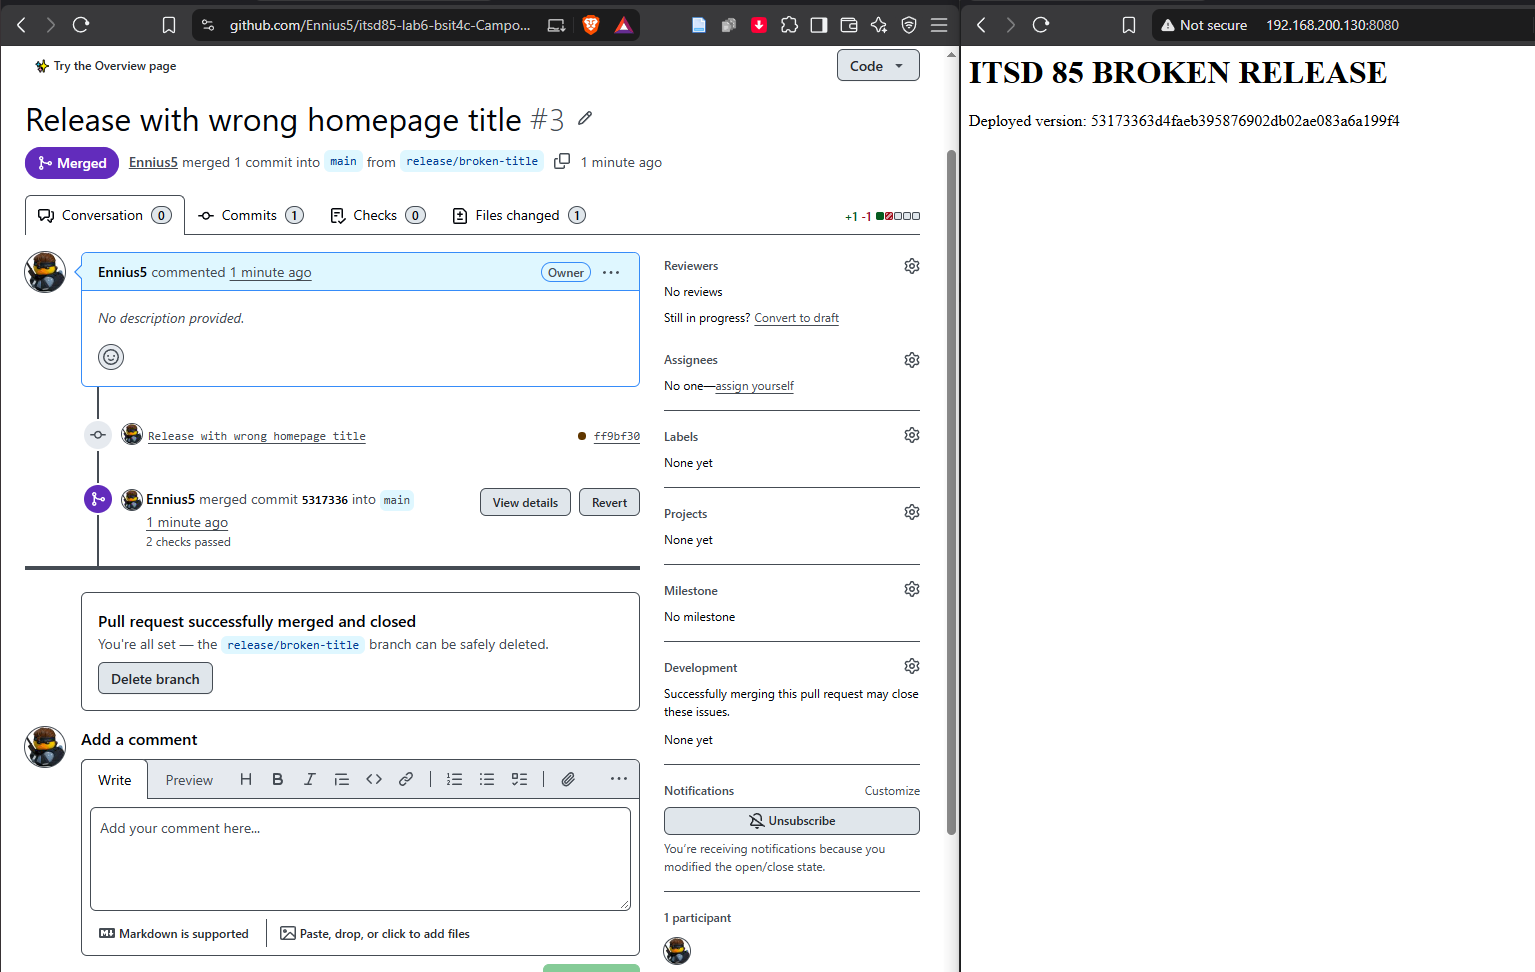
\includegraphics[width=0.95\textwidth]{t7c-broken-live.png}\caption{Test C: the faulty release (wrong title) was merged and deployed.}\label{fig:t7c1}\end{figure}
\begin{figure}[H]\centering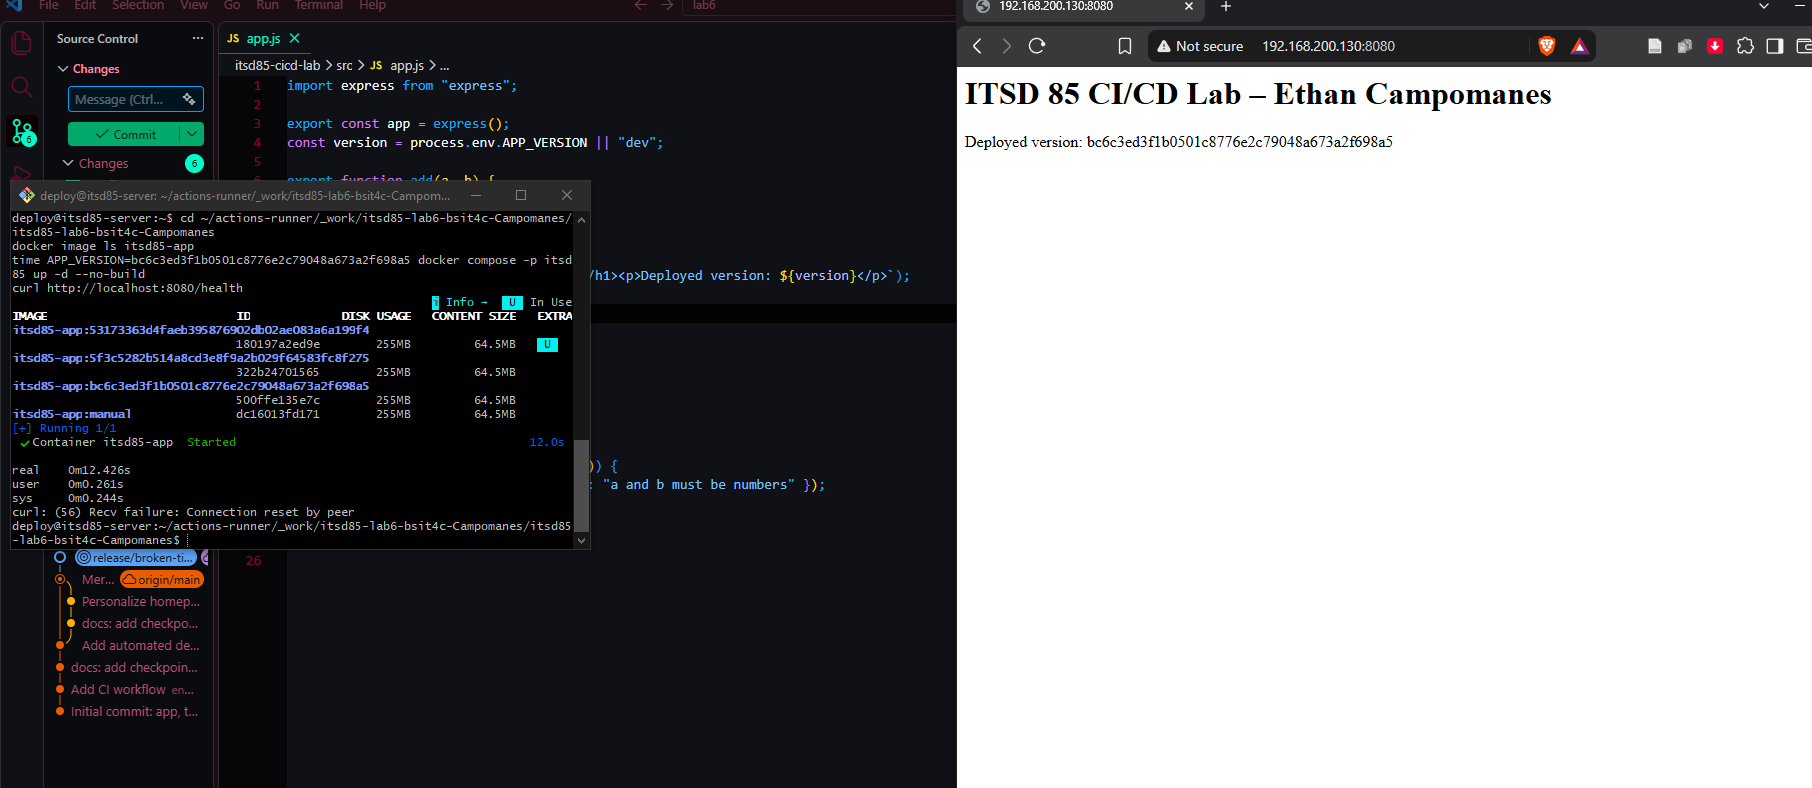
\includegraphics[width=0.95\textwidth]{t7c-method2-rollback.png}\caption{Test C, Method 2: the previous commit's image restarted in 12.4~s.}\label{fig:t7c2}\end{figure}
\begin{figure}[H]\centering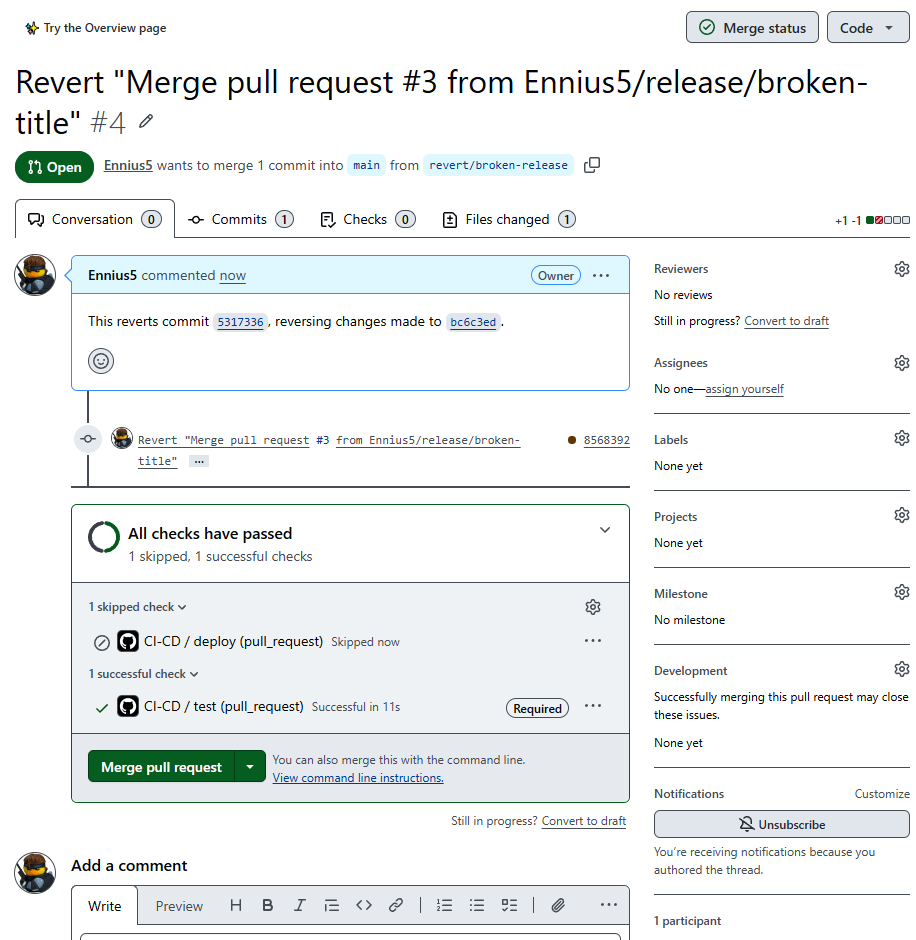
\includegraphics[width=0.7\textwidth]{t7c-revert-pr-green.png}\caption{Test C, Method 1: revert pull request with a passing test check.}\label{fig:t7c3}\end{figure}
\begin{figure}[H]\centering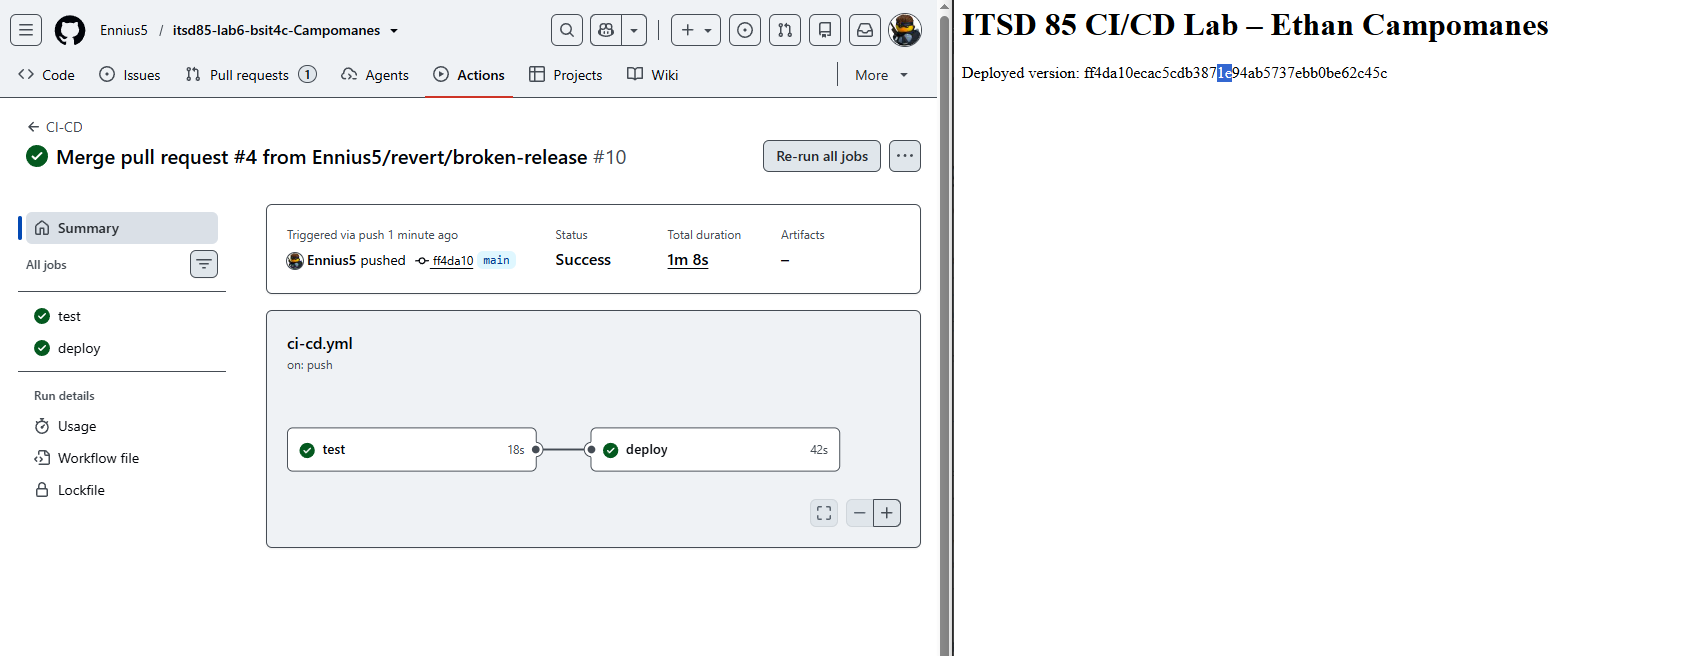
\includegraphics[width=0.95\textwidth]{t7c-method1-revert.png}\caption{Test C, Method 1: the revert deployed as a new version.}\label{fig:t7c4}\end{figure}

\end{document}
